\documentclass[11pt]{article}

\usepackage{graphicx}
%\usepackage{algorithmic}
%\usepackage{algorithm}
\usepackage{amssymb}
\usepackage{amsmath}
\usepackage[mathscr]{euscript}
\usepackage{mathtools}
\usepackage{amsmath}

\begin{document}

\pagenumbering{arabic}

\begin{center}
{\LARGE{\textbf{Uncertainty in Artificial Intelligence}}} \\
\Large\textsc{Ph.D. Comprehensive Exam} \\[1em]
\large\textnormal{Mohammad Shayganfar - mshayganfar@wpi.edu} \\
\large\textnormal{May, 26 2015}
\end{center}

\section{Introduction to Uncertainty in AI}

\section{Sources and Types of Uncertainties}

-Sources:

+ Noise (imprecise observation)

+ Uncertain Change (unprediatable or stochastis behavior of the world)

+ Incompleteness or igonorance (missing information)

\section{Theories of Uncertainties}

\subsection{Bayesian Networks}

\subsubsection{Types of Reasoning}

\subsubsection{Probability Theory}

\subsection{Dempster-Shafer Theory}

In \cite{dempster:theory}, Dempster proposed a probabilistic framework based on
lower and upper bounds on probabilities. In \cite{shafer:evidence-theory},
Shafer developed a formalism for reasoning under uncertainty which uses some of
Dempster's mathematical expressions with different interpretation. Based on
Shafer's formalism, each piece of evidence may support a subset containing
several hypotheses. This is a generalization of the pure probabilistic framework
in which every finding corresponds to a value of a variable (a single
hypothesis) \cite{diez:reasoning-uncertainty}. Therefore, Dempster-Shafer theory
is the generalization of the Bayesian theory of subjective probability to
combine accumulative evidence or to change prior opinions in the light of new
evidence \cite{das:decision-making-agents}. Dempster-Shafer theory is designed
to deal with the distinction between uncertainty and ignorance. Rather than
computing the probability of a proposition, it computes the probability that the
evidence supports the proposition \cite{russell:ai-modern}, and it does not
require the assumption that \textit{Belief}(A) + \textit{Belief}($\neg$A) = 1.
Dempster-Shafer theory deals with the possible values of an unknown variable,
just as deos the theory of probability \cite{tanimoto:ai-lisp}.

There are three basic functions in the Dempster-Shafer theory that we need to
understand for modeling purposes, \textit{mass function, belief function}, and
\textit{plausibility function}. Let $\Theta=\{h_1,h_2, \ldots, h_n\}$ be a
finite set of hypotheses. This set of hypotheses is also called \textit{frame of
discerntment}. The hypotheses represent all the possible states of the system
considered. The set of all subsets of $\Theta$ is its \textit{power set}:
$2^\Theta$. A subset of these $2^\Theta$ sets may consist of a single hypothesis
or of a conjunction of several hypotheses (e.g., a snowy day and a dry day). The
pieces of evidence are events that occurred or may occur (e.g., high pressure
shown by a barometer, or low temprature). One piece of evidence can be related
to a single hypothesis or a set of hypotheses. However, it is not allowed to
have different pieces of evidence lead to the same hypothesis or set of
hypotheses. In fact, the relation between a piece of evidence and a hypothesis
corresponds to a cause-effect chain, i.e., a piece of evidence implies a
hypothesis or a set of hypotheses \cite{kay:dst-reliability}. Moreover, it is
required that all hypotheses are unique, not overlapping and mutually exclusive.

\subsubsection{Mass Function}

A \textit{Basic Probability Assignment} (BPA) or \textit{mass function}
is a function $m:2^\Theta\rightarrow[0,1]$ such that:\\

\textit{m}($\emptyset$) = 0, and $\sum\limits_{x\in2^\Theta}m(x) =1$.\\

The value 0 indicates no belief and the value 1 indicates total belief, and
any value between these two indicate partial belief. As you see the mass
function uses the notion of $2^\Theta$ to be able to use all possible subsets of
the \textit{frame of discernment} $\Theta$. All of the assigned probabilities
sum to unity. There is no belief in empty set. Any subset x of the frame of
discernment $\Theta$ for which m(x) is non-zero is called a \textit{focal
element} and represents the exact belief in the proposition depicted by x. Thus,
any subset is proposition and vice versa. Other elements in Dempster-Shafer
theory are defined by mass function. 

\subsubsection{Belief Function}

Now, we can define another important notion in Dempster-Shafer theory, the
\textit{belief function} (sometimes called a \textit{support function}). It is
the measure of total belief committed to $A \subseteq \Theta$ that can be
obtained by simply adding up the mass of all the subsets of \textit{A}. In other
words, given the frame of discernment $\Theta$ and $A \subseteq \Theta$, the
belief in \textit{A}, denoted \textit{Belief}(\textit{A}), is a number in the
interval [0, 1]. Belief in a set of elements, say \textit{A}, of a frame
$\Theta$, represents the total belief that one has based on the evidence
obtained. Unlike probability theory, \textit{Belief}(\textit{A}) = 0 represents
lack of evidence about \textit{A}, while \textit{p}(A) = 0 represents the
impossibility of \textit{A}. However, \textit{Belief}(\textit{A}) = 1 represents
certainty, that is \textit{A} is certain to occur, similar to \textit{p}(A) = 1,
which also represents the certainty that \textit{A} is true. A belief function
defined on a space $\Theta$ must satisfy the following three properties:

\begin{itemize}
	\item[]\textit{Belief}($\emptyset$) = 0
	\item[]\textit{Belief}($\Theta$) = 1
	\item[]\small\textit{Belief}($A_1 \cup \ldots A_n$)
	$\geq \sum\limits_i\textit{Belief}$($A_i$) - $\sum\limits_{i \textless
	j}\textit{Belief}$($A_i \cap A_j$) + \ldots +\\
	$(-1)^{n+1}\textit{Belief}$($A_i \cap \ldots \cap A_n$)
\end{itemize}

\noindent A belief function is a function $Belief:2^\Theta\rightarrow[0,1]$ and
is defined by:\\

\textit{Belief}(\textit{A}) = $\sum\limits_{B \subseteq A}m(B)\qquad$ for all $A
\subseteq \Theta$\\

\subsubsection{Plausibility Function}

Plausibility in a set, say \textit{A} of a frame $\Theta$ consisting of a
mutually exclusive and exhaustive set of elements, represents the maximum
possibility that a set \textit{A} is true given all the evidences. A
plausibility function \textit{Plausible} defined on a space $\Theta$ must satisfy the
following three properties:

\begin{itemize}
	\item[]\textit{Plausible}($\emptyset$) = 0
	\item[]\textit{Plausible}($\Theta$) = 1
	\item[]\small\textit{Plausible}($A_1 \cap \ldots A_n$)
	$\leq \sum\limits_i\textit{Plausible}$($A_i$) - $\sum\limits_{i \textless
	j}\textit{Plausible}$($A_i \cup A_j$) + \ldots +\\
	$(-1)^{n+1}\textit{Plausible}$($A_i \cup \ldots \cup A_n$)
\end{itemize}

A \textit{plausibility} measure is a function
$Plausible:2^\Theta\rightarrow[0,1]$, and is defined by:\\

\textit{Plausible}(\textit{A}) = $\sum\limits_{B \cap A \neq
\emptyset}m(B)\qquad$ for all $A \subseteq \Theta$\\

\noindent \textit{Plausible}(\textit{A}) in a subset \textit{A} is defined to
be the sum of all mass functions for the subsets \textit{B} that have non-zero
intersections with \textit{A}, and it represents the extent to which we fail to
disbelieve \textit{A}. In other words, it corresponds to the total belief that
does not contradict \textit{A}. The plausibility and belief functions are
related to one another, and we can represent this relation as:\\

\noindent\textit{Belief}(\textit{A}) = 1 -
\textit{Plausible}(\textit{$\neg$A}) $\quad$ and $\quad$
\textit{Plausible}(\textit{A}) = 1 - \textit{Belief}(\textit{$\neg$A}),\\

\noindent where \textit{$\neg$A} is \textit{A}'s complement. Also,
\textit{Belief}(\textit{$\neg$A}) is often called the \textit{doubt} in
\textit{A}. It is noteworthy to mention that Dempster-Shafer theory allows the
representation of \textit{ignorance} since \textit{Belief}(\textit{A}) = 0 does
not imply \textit{Belief}(\textit{$\neg$A}) $\textgreater$ 0 even though
\textit{Belief}(\textit{$\neg$A}) = 1 implies \textit{Belief}(\textit{A}) = 0. Other
notable relations are:\\

\noindent\textit{Belief}(\textit{A}) + \textit{Belief}(\textit{$\neg$A}) $\leq$ 1,
and\\

\noindent\textit{Plausible}(\textit{A}) +
\textit{Plausible}(\textit{$\neg$A}) $\geq$ 1.\\

Here, we also note that in the case of each of the focal elements being
singletons then we return back to traditional Bayesian analysis incorporating
normal probability theory, since in this case \textit{Belief}(\textit{A}) =
\textit{Plausible}(\textit{A}) \cite{beynon:dst-alternative-decision}.

\begin{figure}[tbh]
  \center
  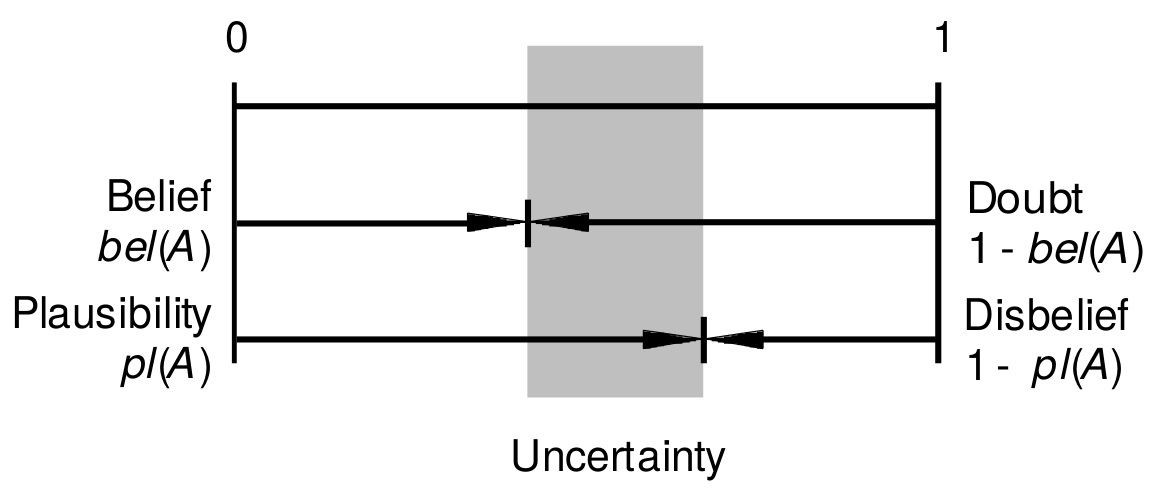
\includegraphics[width=0.65\textwidth]{figure/uncertainty.png}
  \caption{Measures of belief and plausibility. The uncertainty interval is
  shaded gray. \cite{kay:dst-reliability}.}
  \label{fig:uncertainty}
\end{figure}

Collectively the above measures provide Dempster-Shafer theory with an explicit
measure of ignorance about \textit{A} and its complement. All the above measures
of confidence and the BPA are equivalent, in the sense that each of them can be
expressed as a function of any one of the rest. The \textit{uncertainty}
measure is defined as the length of the interval [\textit{Belief}(\textit{A}),
\textit{Plausible}(\textit{A})] where \textit{Belief}(\textit{A}) $\leqslant$
\textit{Plausible}(\textit{A}) \cite{yager:dst-combination-rules}, and it is
also called as \textit{belief interval}. Figure \ref{fig:uncertainty}
illustartes a graphical representation of the belief, plausibility, and doubt
measures which we defined above. As it is shown and said earlier, the difference
between plausibility and belief describes the evidential interval range which
represents the uncertainty concerning the set \textit{A}. Also, as we see in
Figure \ref{fig:uncertainty}, lack of belief does not imply disbelief, since the
complements of belief and plausibility are doubt and disbelief, respectuvely.
Furthermore, the mass assigned to $\Theta$ can be interpreted as the global
ignorance, since the level of mass value is not discernible among the
hypotheses.

\subsubsection{Dempster's Rule of Combination}

Suppose that we have two pieces of uncertain evidence relevant to the same frame of
discerntment $\Theta$. Dempster-Shafer theory also provides a method to combine
the measures of evidence from different sources, using Dempster's rule of
combination which combines two pieces of evidence into a single new piece. The
rule assumes that the sources are independent. If $m_1$ and $m_2$ are the BPA's
associated with $Bel_1$ and $Bel_2$ respectively and $Bel_1$ and $Bel_2$ are
independent, then Dempster's rule of combination is as follows:\\

\[
	[m_1 \oplus m_2](y) = 
    \begin{dcases}
      0, & y = \emptyset \\
      \frac{\sum\limits_{A \cap B = y}m_1(A)m_2(B)}{1-\sum\limits_{A
      \cap B \neq \emptyset}m_1(A)m_2(B)}, & y
      \neq
      \emptyset
	\end{dcases}
\]\\

\noindent The numerator, i.e., $\sum\limits{_{A \cap B =y}}m_1(A)m_2(B)$,
represents the accumulated evidence for the sets A and B, which supports the
given hypothesis y. The denominator in the Dempster's rule of combination, i.e.,
$1-\sum\limits{_{A \cap B \neq \emptyset}}m_1(A)m_2(B)$, is an important
normalization factor denoted by $\mathcal{K}$ which can be interpreted as a
measure of conflict between the sources
\cite{srivastava:evidential-reasoning-uncertainty}.

\subsection{Fuzzy Logic Theory}

Fuzzy Logic provides a mathematical framework to capture uncertainty, and it was
introduced by Zadeh in 1965 \cite{zadeh:fuzzy}. There are different kinds of
uncertainties in the real world. For instance, randomness is one kind, which is
typically modeled using probability theory. Fuzziness manipulates uncertainty by
dealing with the boundaries of a set that are not clearly defined. Fuzzy Logic
is a multivalued logic, that allows intermediate values to be defined between
conventional evaluations like ``true'' and ``false''. Fuzzy Logic's ultimate
goal is to provide foundations for approximate reasoning using imprecise
propositions based on fuzzy set theory. In order to deal with such imprecise
inference, Fuzzy Logic allows the imprecise linguistic terms such as:
fuzzy predicates (e.g., old, expensive), fuzzy quantifiers (e.g., many, little),
and fuzzy truth values (e.g., unlikely false or unlikely true). Fuzzy Logic is a
method for reasoning with logical expressions describing membership in fuzzy
sets \cite{russell:ai-modern}. Logics as bases for reasoning can be
distinguished essentially by three items: truth values, operators, and reasoning
procedures (e.g., tautologies) \cite{zimmermann:fuzzy-sets}. For instance, in
dual logic, truth values can be ``true'' (1) or ``false'' (0), operators can be
defined using the truth tables, and modus ponens or contrapositions can be
considered as tautology. In Fuzzy Logic, the truth values are no longer
restricted to two values, but are expressed by the linguistic variables such as
``true" or ``false". In all forms of fuzzy reasoning, the implications can be
modeled in different ways.

\begin{figure}[tbh]
  \center
  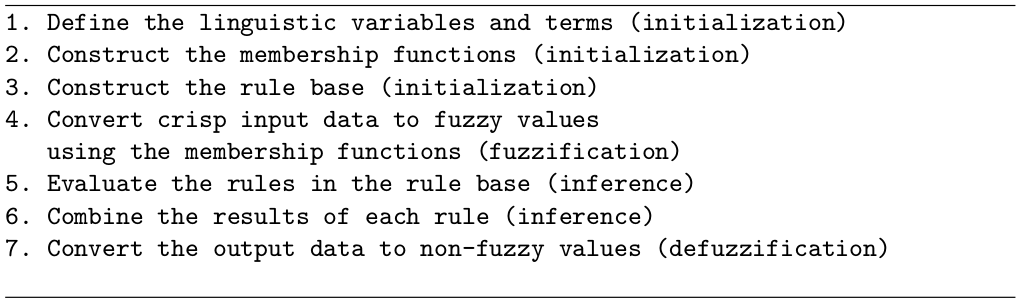
\includegraphics[width=0.95\textwidth]{figure/fuzzy-algorithm.png}
  \caption{Fuzzy Logic algorithm.}
  \label{fig:fuzzy-algorithm}
\end{figure}

Figure \ref{fig:fuzzy-algorithm} shows the Fuzzy Logic algorithm. It begins
with initialization of linguistic varibales (see Section
\ref{sec:linguistic-variables}) and constructing appropriate membership
functions (see Section \ref{sec:membership-function}) and rule-base of the
fuzzy system (see Section \ref{sec:fuzzy-rules}). The constructed membership
functions transfer the input data to fuzzy values (see Section
\ref{sec:fuzzification}). Then, the inference system evaluates the constructed
rules with respect to the given input value, and merges the results obtained
from each rule. Finally, the ovelall result will be transfered to a non-fuzzy
(scalar) value (see Section \ref{sec:defuzzification}).

\subsubsection{Probability vs Possibility}

The theory of possibility is analogous and yet conceptually different from the
theory of probability. Based on the Fuzzy Logic theory of Zadeh
\cite{zadeh:fuzzy} there is a difference between possibility of an event
happening and the probability of that. The follwing example by Zimmermann in
\cite{zimmermann:fuzzy-sets} shows the differnce. Consider the statement ``Hans
ate \textit{X} eggs for breakfast'', where \textit{X} $\in$ \textit{U} = $\{1,
2, \ldots, 8\}$. We may associate a probability \textit{p} by observing
\textit{Hans} eating breakfast for 100 days,

\begin{figure}[tbh]
  \center
  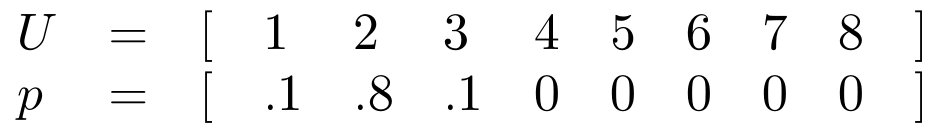
\includegraphics[width=0.65\textwidth]{figure/prob-poss-01.png}
  \label{fig:probability}
\end{figure}

A fuzzy set expressing the degree to which \textit{Hans} can eat \textit{X} eggs
in breakfast may be the following possibilty distribution $\pi$,

\begin{figure}[tbh]
  \center
  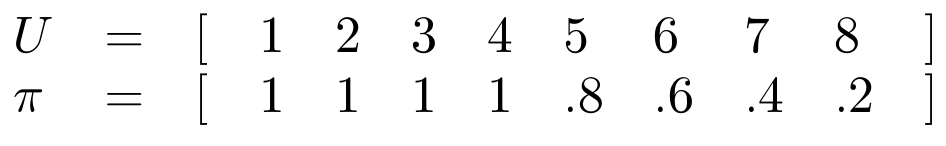
\includegraphics[width=0.65\textwidth]{figure/prob-poss-02.png}
  \label{fig:ppssibility}
\end{figure}

where the possiibility of \textit{X} = 3 is 1, while the probability of
\textit{Hnas} eating 3 eggs for breakfast is only 0.1. Therefore, the example
shows, that a possible event does not necessarily imply that it is probable too.
However, if the event is probable it must also be possible
\cite{zimmermann:fuzzy-sets}.

\subsubsection{Membership Functions}
\label{sec:membership-function}

The difference between crisp (i.e., classical) and fuzzy sets is established by
introducing a \textit{membership function}. Membership functions are
mathematical tools for indicating flexible membership to a set, modeling and
quantifying the meaning of symbols. Membership functions are used in the
fuzzification and defuzzification steps (see Sections \ref{sec:fuzzification}
and \ref{sec:defuzzification}) of a Fuzzy Logic system. A membership function is
used to quantify a linguistic term (see Section \ref{sec:linguistic-variables}).
Therefore, the manipulation of fuzzy quantities can be accomplished by
manipulation of fuzzy set membership functions. Some of the manipulation
includes set complement, intersection, and union as well as fuzzification and
defuzzification (see Sections \ref{sec:fuzzification} and
\ref{sec:defuzzification}) \cite{schalkoff:intelligent-systems}.

\begin{figure}[tbh]
  \center
  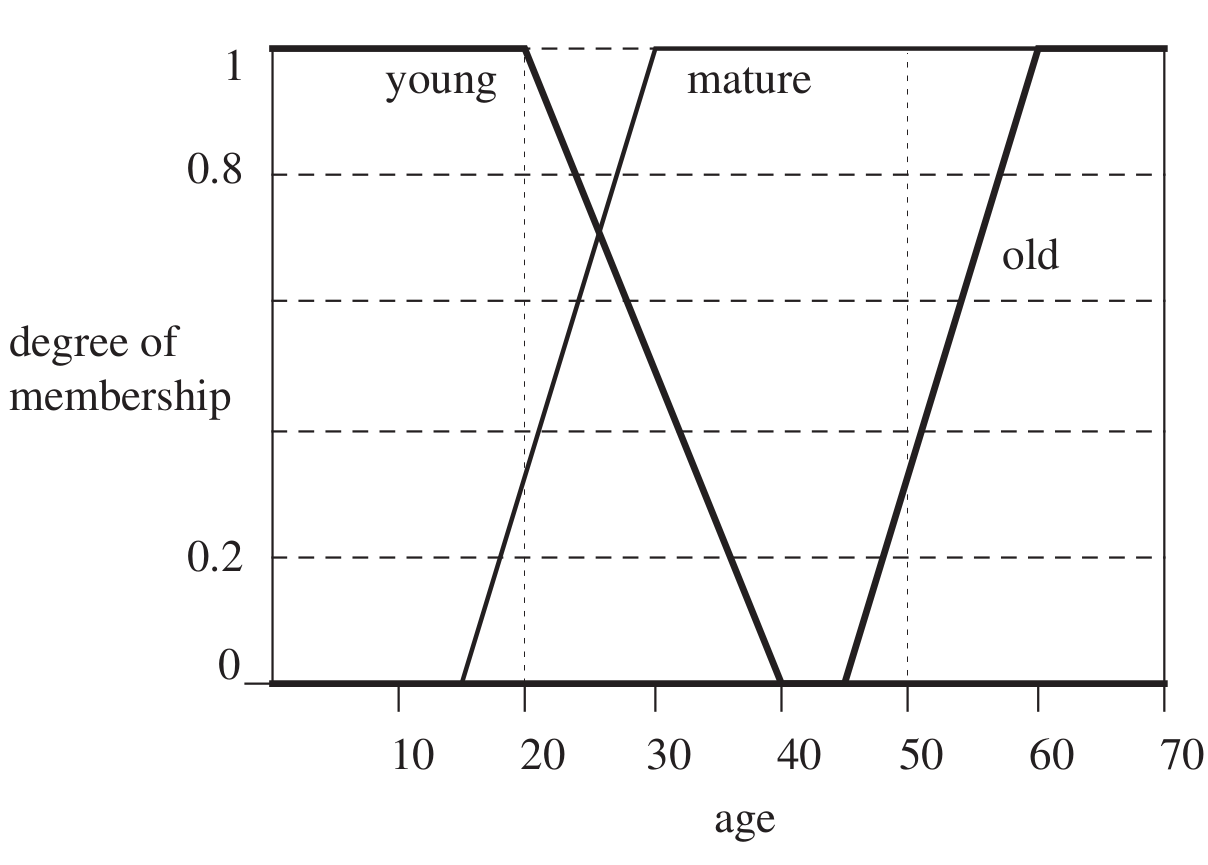
\includegraphics[width=0.65\textwidth]{figure/membership-function.png}
  \caption{Membership functions for the concepts young, mature and old.}
  \label{fig:membership-function}
\end{figure}

Figure \ref{fig:membership-function} shows membership functions for three
linguistic terms of age variable. It shows three examples of a membership
functions in the interval 0 to 70 years. These three functions define the degree
of membership of any given age in the sets of young, mature, and old ages.
Note that, an important characteristic of fuzzy logic is that a numerical value
does not have to be fuzzified using only one membership function. In other
words, a value can belong to multiple sets at the same time. For insatnce, if
someone is 20 years old her degree of membership in the set of young persons is
1.0 (maximum value), in the set of adults 0.35, and in the set of old persons
0.0 (minimum value). As another example, if someone is 50 years old the degrees
of membership in the sets of young, mature, and old are 0.0, 1.0, 0.3
respectively.

The membership function is a graphical representation of the magnitude of
participation of each input. It associates a weighting with each of the inputs
that are processed, define functional overlap between inputs, and ultimately
determines an output response.

Let $\mathcal{X}$ be a classical universal set. A fuzzy subset $\textit{A}$ of
$\mathcal{X}$ is characterized by a \textit{membership function}: $\mu_A$ :
$\mathcal{X} \rightarrow$ [0, 1]. $\mu_A$($\textit{x}$) is called the
\textit{membership degree (grade)} of $\textit{x}$ in $\textit{A}$. The degree
of membership is expressed by a real number in the interval [0, 1]. The degree
of membership is a precise, but subjective measure that depends on the context.
The followings define some of the important properties of membership function.\\

\textbf{Height:} The height of $\textit{A}$, denoted by
$\textit{h}$($\textit{A}$), corresponds to the upper bound of the membership
function:\\ \\$\textit{h}$($\textit{A}$) = sup$\{\mu_A(\textit{x}) | \textit{x}
\in \mathcal{X}\}$.\\

\textbf{Support:} The support of $\textit{A}$ is a set of all elements
\textit{x} of $\mathcal{X}$ for which (\textit{x}, $\mu_A$(\textit{x})) $\in$
$\textit{A}$ and $\mu_A$(\textit{x}) $\textgreater$ 0 holds. In other words,
support is a set of elements that have a non-zero membership.\\

\textbf{$\alpha$-cut:} An $\alpha$-cut of $\textit{A}$ is the subset of elements
with a membership degree greater than or equal to $\alpha$. The $\alpha$-cut is
denoted by:\\ \\$\alpha$-cut($\textit{A}$) = $\{\textit{x} \in \mathcal{X} |
\mu_A(\textit{x}) \geqslant \alpha\}$.\\

\textbf{kernel:}

Membership functions can have different shapes and their shape can be determined
arbitrarilty based on experience or by running statistical studies on data.
They can be sigmoidal, heyperbolic, Gaussian or any other shape.

The rules use the input membership values as weighting factors to determine
their influence on the fuzzy output sets of the final output conclusion.

\subsubsection{Linguistic Variables}
\label{sec:linguistic-variables}

The concept of membership function discussed in Section
\ref{sec:membership-function} allows us to define fuzzy systems in natural
language. Linguistic variables are the input or output variables of the system
whose values are words or sentences from a natural language, instead of
numerical values. In fact, just like an algebraic variable takes numbers as
values, a linguistic variable takes words or sentences as values
\cite{zimmermann:fuzzy-sets}. A linguistic variable is generally decomposed into
a set of linguistic terms. For instance, for people's age, we usually use terms
such as ``old'' or ``young'' which are called linguistic values of the age.
Then, we can consider a set of decompositions for the linguistic variable age,
\textit{Height}(\textit{h}) = {very-old, old, mature, young, very-young}. The
members of this decomposition set are called \textit{linguistic terms} which can
cover a portion of the overall values of people's age. In other words, the
values that a linguistic variable can take is called its linguistic terms.

\subsubsection{Fuzzy Operators}

Fuzzy operators are used in order to manipulate fuzzy sets, and for being able
to evaluate the constructed fuzzy rules, and ultimately to be able to combine
the results of the individual rules. The operations on fuzzy sets are different
than the operations on classical sets. The definitions of operators on fuzzy
sets are not the same and can be chosen. Zadeh in \cite{zadeh:fuzzy} defined the
intersection (logical and), union (exclusive or), and complement (negation)
operations for fuzzy sets as generalization of crisp sets and of crisp
statements. Here are the two sets of operators for the complement (NOT), the
intersection (AND) and union (OR) most commonly used:\\

\noindent The memebership function of the \textbf{Intersection} of two fuzzy
sets \textit{A} and \textit{B}:\\

$\mu_{A \cap B}(X)$ = Min($\mu_{A}(X), \mu_{B}(X)$) $\qquad \forall x \in X$\\

\noindent The memebership function of the \textbf{union} of two fuzzy sets
\textit{A} and \textit{B}:\\

$\mu_{A \cup B}(X)$ = Max($\mu_{A}(X), \mu_{B}(X)$) $\qquad \forall x \in X$\\

\noindent The memebership function of the \textbf{complement} of a fuzzy set
\textit{A}:\\

$\mu_{A}(X)$ = 1 - $\mu_{A}(X) \qquad \forall x \in X$\\

\noindent These definitions were later extended by other reasearchers too, e.g.,
\cite{yager:generalizing-leximin}.

\subsubsection{Fuzzy Sets}

Fuzzy sets are a further development of the mathematical concept of a
conventional set. A fuzzy set is a class of objects with continuum of
degrees of membership \cite{zadeh:fuzzy}. Following Zadeh \cite{zadeh:fuzzy}
many sets have more than an either-or criterion for membership. For insatnce,
the set young people which can contain people at diffrent ages. A fuzzy set
$\textit{A}$ is defined by a membership function $\mu_A$ from the universe of
discourse $X_i$ to the closed unit interval [0,1]. We interpret
$\mu_A$($\textit{x}$) as the degree of membership of $\textit{x}$ in \textit{A}.
Zadeh proposed this degree of membership, such that the transition from
membership to non-membership is gradual rather than abrupt. Therefore, the
degree of membership for all its members describes a fuzzy set.

\subsubsection{Fuzzy Rules}
\label{sec:fuzzy-rules}

In a Fuzzy Logic system, a rule-base is constructed to determine and control the
output variable. Fuzzy rules are simply comprised of IF-THEN rules which include
two parts of condition and conclusion. A fuzzy rule is encoded in a statement in
the following form:\\

\noindent \textbf{IF} (a statement of conditions is satisfied)

$\qquad\qquad\qquad\qquad\qquad$\textbf{THEN} (a set of consequences can
be inferred).\\

The followings are two examples of fuzzy
rules based on the age example depicted in Figure
\ref{fig:membership-function}:\\

\textbf{IF} (age is \textit{young}) \textbf{THEN} (run \textit{command
``talk''})
 
\textbf{IF} (age is \textit{old} \textbf{OR} \textit{mature}) \textbf{THEN} (run
\textit{command ``listen''})

\subsubsection{Fuzzification}
\label{sec:fuzzification}

The fuzzification process is mainly used to transform a crisp set to a fuzzy
set. A fuzzifier function F is used to control the fuzziness of the set.

\subsubsection{Inference in Fuzzy Logic}
\label{sec:reasoning}

In order to draw conclusions from a rule-base we need a mechanism that can
produce an output from a collection of IF-THEN rules. Meaning, after evaluating
the result of each rule with respect to the given input value(s), the results of
the rules should be combined to obtain a final result. This process in Fuzzy
Logic systems is called inference. The results of individual rules can be
combined in different ways. There are different types of accumulation methods
that can be used to combine the results id individual rules.

\subsubsection{Defuzzification}
\label{sec:defuzzification}

After the inference step, the Fuzzy Logic system provides the overall result as
a fuzzy value. Then, to obtain a final crisp output value, this fuzzy result
should be defuzzified which is the purpose of the defuzzifier component of a
Fuzzy Logic system. Defuzzification is performed according to the membership
function of the output variable. Figure \ref{fig:defuzzification} shows the
defuzzification step of in a Fuzzy Logic system.

\begin{figure}[tbh]
  \center
  \includegraphics[width=0.65\textwidth]{figure/defuzzification.png}
  \caption{Defuzzification step.}
  \label{fig:defuzzification}
\end{figure}

There are different algorithms for defuzzification step. One of the most common
used algorithms is called called center of gravity.

In summary, Figure \ref{fig:fuzzy-system} (see also Figure
\ref{fig:fuzzy-algorithm}) shows the process of fuzzy logic. Firstly, a crisp
set of input data are gathered and converted to a fuzzy set using fuzzy
linguistic variables (see Section \ref{sec:linguistic-variables}), fuzzy
linguistic terms and membership functions (see Section
\ref{sec:membership-function}). This step is known as fuzzification (see
Section \ref{sec:fuzzification}). Afterwards, an inference is made based on a
set of rules (see Section \ref{sec:reasoning}). Lastly, the resulting fuzzy
output is mapped to a crisp output using the membership functions, in the
defuzzification step (see Section \ref{sec:defuzzification}).

\begin{figure}[tbh]
  \center
  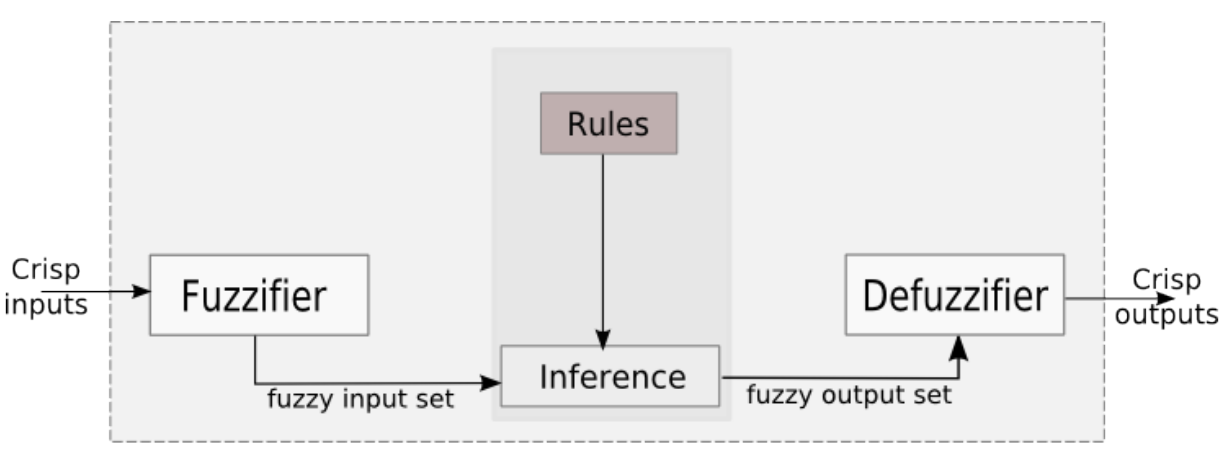
\includegraphics[width=0.85\textwidth]{figure/fuzzy-system.png}
  \caption{A Fuzzy Logic system.}
  \label{fig:fuzzy-system}
\end{figure}

\subsection{Other approaches}

\section{Strengths and Weaknesses}

In general, there is an increasing trend of computational complexity Fuzzy Logic
to probabilistic approaches and Dempster-Shafer theory. However, the
representational power and precision increases in the same order and direction.

- Locality in rule-based systems vs. using all evidences in probabilistic
systems [R\&N AI book p.524]

-Detachment in rule-based systems vs. requiring the source of evidence for
subsequent probabilistic reasoning [R\&N AI book p.524]

- Dempster-Shafer theory allows no definite decision in many cases, whereas
probabilistic inference does yield a specific choice \cite{russell:ai-modern}.

- In contrast to Dempster-Shafer theory, a complete Bayesian model would include
probability estimates for factors that allow us to express the ignorance in
terms of how our beliefs would change in the face of future informaiton
gathering \cite{russell:ai-modern}.

\subsection{Advantages and Disadvantages of Belief Networks}

Like any other computational formalism, belief network technology offers certain
advantages and disadvantages. Advantages of belief networks include
\cite{das:decision-making-agents}:

\begin{itemize}
  \item Sound theoretical foundation: The computation of beliefs using
  probability estimates is guaranteed to be consistent with probability theory.
  This advantage stems from the Bayesian update procedure’s strict derivation
  from the axioms of probability.
  \item Graphical models: Belief networks graphically depict the
  interdependencies that exist between related pieces of domain knowledge,
  enhancing understanding of the domain. The structure of a belief network
  captures the cause-effect relationships that exist amongst the variables of
  the domain. The ease of causal interpretation in belief network models
  typically makes them easier to construct than other models, minimizing the
  knowledge engineering costs and making them easier to modify.
  \item Predictive and diagnostic reasoning: Belief networks combine both
  deductive/predictive and abductive/diagnostic reasoning. Interdependencies
  among variables in a network are accurately captured and speculative if-then
  type computation can be performed.
  \item Computational tractability: Belief networks are computationally
  tractable for most practical applications. This efficiency stems principally
  from the exploitation of conditional independence relationships over the
  domain. We have presented an efficient single-pass evidence propagation
  algorithm for networks without loops.
  \item Evidence handling: Evidence can be posted to any node in a belief
  network. This means that subjective evidence can be posted at an intermediate
  node representing an abstract concept.
\end{itemize}

A major disadvantage of belief network technology is the high level of effort
required to build network models. Although it is relatively easy to build a
belief network structure with the help of subject matter experts, the model will
require a significant amount of probability data as the number of nodes and
links in the structure increase. The size of a CPT corresponding to a node with
multiple parents can potentially be huge. For example, the number of independent
entries in the CPT of a binary node (a node with two states) with 8 binary
parent variables is 128.

Belief networks are also poor at handling continuous variables. Current
software handles continuous variables in a very restrictive manner (for example,
they must be Gaussian and can only be children). Lener et al. (2001) developed
an inference algorithm for static hybrid belief networks, which are Conditional
Linear Gaussian models, where the conditional distribution of the continuous
variables assigned to the discrete variables is a multivariate Gaussian. Cob and
Shenoy (2004) developed an inference algorithm in hybrid belief networks using
Mixtures of Truncated Potentials. But these techniques are yet to be incorporated
in commercial software.

\subsection{Advantages and Disadvantages of Dempster-Shafer Theory}

- Its ability to represent ignorance in a direct and straightforward fashion.

- Its consistency with classical probability theory.

- Its manageable computational complexity.

- Represents the actual state of belief more precisely

- Distinguishes randomness from missing information

- Prior probabilities not required.

Dis:

- Lack of assessment strategies: There is a necessity to assign precise numbers
in Dempster-Shafer theory's applications to each subset $A \subseteq \Theta$ by
the basic assignment m. Although, the precise degrees of the desired measures
may exist, but it is perhaps too difficult to determine them with the necessary
precision.

- Instability: Underlying beliefs may be unstable. Estimated beliefs may be
influenced by the condi- tions of its estimation.

- Ambiguity: Ambiguous or imprecise judgement could not be expressed by the
evidence measures.

- The main problem of the Dempster-Shafer theoryin its original formulation is
that its computational complexity grows exponentially with the number of
hypotheses.

- mathematically complex

- Has to be calculated over all possible sets of states

- A small modification of the evidence assignments may lead to a completely
different conclusion.

- Can lead to misleading and counter-intuitive results.

\subsection{Advantages and Disadvantages of Fuzzy Logic}

- Easy to design 

- Relatively intuitive rules 

- Relatively robust controllers 

Dis:

- Verification and validation of a fuzzy knowledge-based is typically expensive.

- Determining the exact fuzzy rules and membership functions is a hard task
(it is difficult to determine or predict the required number of membership
functions).

- Stability is an important concern for fuzzy systems.

- Longer inference chains can be problematic 

- The order of inference steps matters

- After inference it can be difficult to exactly interpret the membership value 


\section{Applications of Bayesian Networks}

\section{Conclusion}

\bibliographystyle{plain}
\bibliography{mshayganfar}

\end{document}